\documentclass[]{article}
\usepackage{lmodern}
\usepackage{amssymb,amsmath}
\usepackage{ifxetex,ifluatex}
\usepackage{fixltx2e} % provides \textsubscript
\ifnum 0\ifxetex 1\fi\ifluatex 1\fi=0 % if pdftex
  \usepackage[T1]{fontenc}
  \usepackage[utf8]{inputenc}
\else % if luatex or xelatex
  \ifxetex
    \usepackage{mathspec}
  \else
    \usepackage{fontspec}
  \fi
  \defaultfontfeatures{Ligatures=TeX,Scale=MatchLowercase}
\fi
% use upquote if available, for straight quotes in verbatim environments
\IfFileExists{upquote.sty}{\usepackage{upquote}}{}
% use microtype if available
\IfFileExists{microtype.sty}{%
\usepackage{microtype}
\UseMicrotypeSet[protrusion]{basicmath} % disable protrusion for tt fonts
}{}
\usepackage[margin=1in]{geometry}
\usepackage{hyperref}
\hypersetup{unicode=true,
            pdftitle={Statistical Inference \textbar{} Simulation Excercise},
            pdfauthor={Alex Lee},
            pdfborder={0 0 0},
            breaklinks=true}
\urlstyle{same}  % don't use monospace font for urls
\usepackage{color}
\usepackage{fancyvrb}
\newcommand{\VerbBar}{|}
\newcommand{\VERB}{\Verb[commandchars=\\\{\}]}
\DefineVerbatimEnvironment{Highlighting}{Verbatim}{commandchars=\\\{\}}
% Add ',fontsize=\small' for more characters per line
\usepackage{framed}
\definecolor{shadecolor}{RGB}{248,248,248}
\newenvironment{Shaded}{\begin{snugshade}}{\end{snugshade}}
\newcommand{\AlertTok}[1]{\textcolor[rgb]{0.94,0.16,0.16}{#1}}
\newcommand{\AnnotationTok}[1]{\textcolor[rgb]{0.56,0.35,0.01}{\textbf{\textit{#1}}}}
\newcommand{\AttributeTok}[1]{\textcolor[rgb]{0.77,0.63,0.00}{#1}}
\newcommand{\BaseNTok}[1]{\textcolor[rgb]{0.00,0.00,0.81}{#1}}
\newcommand{\BuiltInTok}[1]{#1}
\newcommand{\CharTok}[1]{\textcolor[rgb]{0.31,0.60,0.02}{#1}}
\newcommand{\CommentTok}[1]{\textcolor[rgb]{0.56,0.35,0.01}{\textit{#1}}}
\newcommand{\CommentVarTok}[1]{\textcolor[rgb]{0.56,0.35,0.01}{\textbf{\textit{#1}}}}
\newcommand{\ConstantTok}[1]{\textcolor[rgb]{0.00,0.00,0.00}{#1}}
\newcommand{\ControlFlowTok}[1]{\textcolor[rgb]{0.13,0.29,0.53}{\textbf{#1}}}
\newcommand{\DataTypeTok}[1]{\textcolor[rgb]{0.13,0.29,0.53}{#1}}
\newcommand{\DecValTok}[1]{\textcolor[rgb]{0.00,0.00,0.81}{#1}}
\newcommand{\DocumentationTok}[1]{\textcolor[rgb]{0.56,0.35,0.01}{\textbf{\textit{#1}}}}
\newcommand{\ErrorTok}[1]{\textcolor[rgb]{0.64,0.00,0.00}{\textbf{#1}}}
\newcommand{\ExtensionTok}[1]{#1}
\newcommand{\FloatTok}[1]{\textcolor[rgb]{0.00,0.00,0.81}{#1}}
\newcommand{\FunctionTok}[1]{\textcolor[rgb]{0.00,0.00,0.00}{#1}}
\newcommand{\ImportTok}[1]{#1}
\newcommand{\InformationTok}[1]{\textcolor[rgb]{0.56,0.35,0.01}{\textbf{\textit{#1}}}}
\newcommand{\KeywordTok}[1]{\textcolor[rgb]{0.13,0.29,0.53}{\textbf{#1}}}
\newcommand{\NormalTok}[1]{#1}
\newcommand{\OperatorTok}[1]{\textcolor[rgb]{0.81,0.36,0.00}{\textbf{#1}}}
\newcommand{\OtherTok}[1]{\textcolor[rgb]{0.56,0.35,0.01}{#1}}
\newcommand{\PreprocessorTok}[1]{\textcolor[rgb]{0.56,0.35,0.01}{\textit{#1}}}
\newcommand{\RegionMarkerTok}[1]{#1}
\newcommand{\SpecialCharTok}[1]{\textcolor[rgb]{0.00,0.00,0.00}{#1}}
\newcommand{\SpecialStringTok}[1]{\textcolor[rgb]{0.31,0.60,0.02}{#1}}
\newcommand{\StringTok}[1]{\textcolor[rgb]{0.31,0.60,0.02}{#1}}
\newcommand{\VariableTok}[1]{\textcolor[rgb]{0.00,0.00,0.00}{#1}}
\newcommand{\VerbatimStringTok}[1]{\textcolor[rgb]{0.31,0.60,0.02}{#1}}
\newcommand{\WarningTok}[1]{\textcolor[rgb]{0.56,0.35,0.01}{\textbf{\textit{#1}}}}
\usepackage{graphicx,grffile}
\makeatletter
\def\maxwidth{\ifdim\Gin@nat@width>\linewidth\linewidth\else\Gin@nat@width\fi}
\def\maxheight{\ifdim\Gin@nat@height>\textheight\textheight\else\Gin@nat@height\fi}
\makeatother
% Scale images if necessary, so that they will not overflow the page
% margins by default, and it is still possible to overwrite the defaults
% using explicit options in \includegraphics[width, height, ...]{}
\setkeys{Gin}{width=\maxwidth,height=\maxheight,keepaspectratio}
\IfFileExists{parskip.sty}{%
\usepackage{parskip}
}{% else
\setlength{\parindent}{0pt}
\setlength{\parskip}{6pt plus 2pt minus 1pt}
}
\setlength{\emergencystretch}{3em}  % prevent overfull lines
\providecommand{\tightlist}{%
  \setlength{\itemsep}{0pt}\setlength{\parskip}{0pt}}
\setcounter{secnumdepth}{0}
% Redefines (sub)paragraphs to behave more like sections
\ifx\paragraph\undefined\else
\let\oldparagraph\paragraph
\renewcommand{\paragraph}[1]{\oldparagraph{#1}\mbox{}}
\fi
\ifx\subparagraph\undefined\else
\let\oldsubparagraph\subparagraph
\renewcommand{\subparagraph}[1]{\oldsubparagraph{#1}\mbox{}}
\fi

%%% Use protect on footnotes to avoid problems with footnotes in titles
\let\rmarkdownfootnote\footnote%
\def\footnote{\protect\rmarkdownfootnote}

%%% Change title format to be more compact
\usepackage{titling}

% Create subtitle command for use in maketitle
\providecommand{\subtitle}[1]{
  \posttitle{
    \begin{center}\large#1\end{center}
    }
}

\setlength{\droptitle}{-2em}

  \title{Statistical Inference \textbar{} Simulation Excercise}
    \pretitle{\vspace{\droptitle}\centering\huge}
  \posttitle{\par}
    \author{Alex Lee}
    \preauthor{\centering\large\emph}
  \postauthor{\par}
      \predate{\centering\large\emph}
  \postdate{\par}
    \date{10/3/2019}


\begin{document}
\maketitle

\hypertarget{overview}{%
\section{Overview}\label{overview}}

The goal of this project is to investigate the relationship between an
exponential distribution (using R) and the Central Limit Theorom (CLR).

We know that the Central Limit Theorom can take in any probability
distribution, given a well-defined mean and variance, and determine the
mean. The mean is obtained by taking a random number of samples in the
distribution and calculating the sample mean. The resulting distribution
is a normal distribution where the mean should near equal to the
original distribution mean.

Exponential Distribution is a probability distribution that determines
the probabilities of events occuring given a specific time unit. This
category of distribtion is (typically) asymmptotic in nature where the
area under the curve be 1.

\hypertarget{simulations}{%
\section{Simulations}\label{simulations}}

The simulation will rely on R to generate a set of random distributions.
The exponential distribution can be simulated in R with rexp(n, lambda)
where lambda is the rate parameter. The mean of exponential distribution
is 1/lambda and the standard deviation is also 1/lambda. Set lambda =
0.2 for all of the simulations. You will investigate the distribution of
averages of 40 exponentials. Note that you will need to do a 1000
simulations.

The below R code initializes the simulation given the parameters above:

\begin{Shaded}
\begin{Highlighting}[]
\KeywordTok{set.seed}\NormalTok{(}\DecValTok{5}\NormalTok{)}
\NormalTok{lambda     <-}\StringTok{ }\FloatTok{0.2}
\NormalTok{n          <-}\StringTok{ }\DecValTok{40}
\NormalTok{sim        <-}\StringTok{ }\DecValTok{1000} 
\NormalTok{exp_data   <-}\StringTok{ }\KeywordTok{replicate}\NormalTok{(sim, }\KeywordTok{mean}\NormalTok{(}\KeywordTok{rexp}\NormalTok{(n, lambda)))}
\end{Highlighting}
\end{Shaded}

In this section, we set the variable lambda (or rate) to 0.2, then
define the number of sample variables to 40, defin the number of
simulations to run and, lastly, use rexp() function to generate our
exponential data distribution and assign it to the exp\_data data frame.

\hypertarget{sample-mean-versus-theoretical-mean}{%
\section{Sample Mean versus Theoretical
Mean}\label{sample-mean-versus-theoretical-mean}}

According to CLT, the sample mean should be roughly close to the
theoretical mean. We will use R to run simple mean calculations against
the exp\_data set and compare it to the theoretical mean (1/lambda).

\begin{Shaded}
\begin{Highlighting}[]
\NormalTok{th_mean    <-}\StringTok{ }\DecValTok{1}\OperatorTok{/}\NormalTok{lambda}
\NormalTok{sim_mean   <-}\StringTok{ }\KeywordTok{mean}\NormalTok{(exp_data)}

\NormalTok{th_mean}
\end{Highlighting}
\end{Shaded}

\begin{verbatim}
## [1] 5
\end{verbatim}

\begin{Shaded}
\begin{Highlighting}[]
\NormalTok{sim_mean}
\end{Highlighting}
\end{Shaded}

\begin{verbatim}
## [1] 5.043053
\end{verbatim}

As expected, the simulated mean (CLT), given a sample set size of 40 and
1000 total samples does provide a very close mean approximation to the
theoretical mean. In this case, the simulated mean returns a mean value
of 5.04 while the theoretical mean gives us 5.0.

\hypertarget{sample-variance-versus-theoretical-variance}{%
\section{Sample Variance versus Theoretical
Variance}\label{sample-variance-versus-theoretical-variance}}

CLT also provides a very close variance approximation when compared to
the theoretical variance. In this case, we calculate the simulated
variance to be 0.602 while the theoretical variance is 0.625.

\begin{Shaded}
\begin{Highlighting}[]
\NormalTok{sim_var    <-}\StringTok{ }\KeywordTok{var}\NormalTok{(exp_data)}
\NormalTok{th_var     <-}\StringTok{ }\DecValTok{1}\OperatorTok{/}\NormalTok{(lambda}\OperatorTok{^}\DecValTok{2}\OperatorTok{*}\NormalTok{n)}

\NormalTok{sim_var }
\end{Highlighting}
\end{Shaded}

\begin{verbatim}
## [1] 0.6026047
\end{verbatim}

\begin{Shaded}
\begin{Highlighting}[]
\NormalTok{th_var}
\end{Highlighting}
\end{Shaded}

\begin{verbatim}
## [1] 0.625
\end{verbatim}

We expect a close variance because of the nature of CLT in how it
produces a normal distribution of sample means, given a large enough
sample set size and number of samples.

\hypertarget{distribution}{%
\section{Distribution}\label{distribution}}

Up until now, we only provided a numerical view of the results. To
better see CLT in action, we need to generate a plot of the sample means
as this relates to a normal distribtuion line. We will also need to
calculate the theoretical standard deviation as part of this plotting
excercise.

\begin{Shaded}
\begin{Highlighting}[]
\KeywordTok{library}\NormalTok{(ggplot2)}

\NormalTok{th_sd   <-}\StringTok{ }\NormalTok{(}\DecValTok{1}\OperatorTok{/}\NormalTok{lambda)}\OperatorTok{/}\KeywordTok{sqrt}\NormalTok{(n)}

\NormalTok{hist   <-}\StringTok{ }\KeywordTok{ggplot}\NormalTok{(}\KeywordTok{data.frame}\NormalTok{(exp_data), }\KeywordTok{aes}\NormalTok{(}\DataTypeTok{x =}\NormalTok{ exp_data)) }
\NormalTok{hist   <-}\StringTok{ }\NormalTok{hist }\OperatorTok{+}\StringTok{ }\KeywordTok{geom_histogram}\NormalTok{(}\KeywordTok{aes}\NormalTok{(}\DataTypeTok{y =}\NormalTok{ ..density..), }\DataTypeTok{colour =} \StringTok{"black"}\NormalTok{, }\DataTypeTok{fill =} \StringTok{"green"}\NormalTok{, }\DataTypeTok{alpha =} \FloatTok{.3}\NormalTok{,}\DataTypeTok{binwidth=}\NormalTok{.}\DecValTok{2}\NormalTok{)}
\NormalTok{hist   <-}\StringTok{ }\NormalTok{hist }\OperatorTok{+}\StringTok{ }\KeywordTok{stat_function}\NormalTok{(}\DataTypeTok{fun =} \StringTok{"dnorm"}\NormalTok{, }\DataTypeTok{args =} \KeywordTok{list}\NormalTok{(}\DataTypeTok{mean =}\NormalTok{ th_mean, }\DataTypeTok{sd =}\NormalTok{ th_sd))}
\NormalTok{hist   <-}\StringTok{ }\NormalTok{hist }\OperatorTok{+}\StringTok{ }\KeywordTok{geom_vline}\NormalTok{(}\DataTypeTok{xintercept=}\NormalTok{th_mean,}\DataTypeTok{size=}\DecValTok{1}\NormalTok{,}\DataTypeTok{colour=}\StringTok{"red"}\NormalTok{)}
\NormalTok{hist   <-}\StringTok{ }\NormalTok{hist }\OperatorTok{+}\StringTok{ }\KeywordTok{xlab}\NormalTok{(}\StringTok{"Mean"}\NormalTok{)}\OperatorTok{+}\KeywordTok{ylab}\NormalTok{(}\StringTok{"Density"}\NormalTok{)}
\NormalTok{hist   <-}\StringTok{ }\NormalTok{hist }\OperatorTok{+}\StringTok{ }\KeywordTok{scale_x_continuous}\NormalTok{(}\DataTypeTok{breaks =} \KeywordTok{c}\NormalTok{(}\DecValTok{1}\OperatorTok{:}\DecValTok{10}\NormalTok{))}
\NormalTok{hist}
\end{Highlighting}
\end{Shaded}

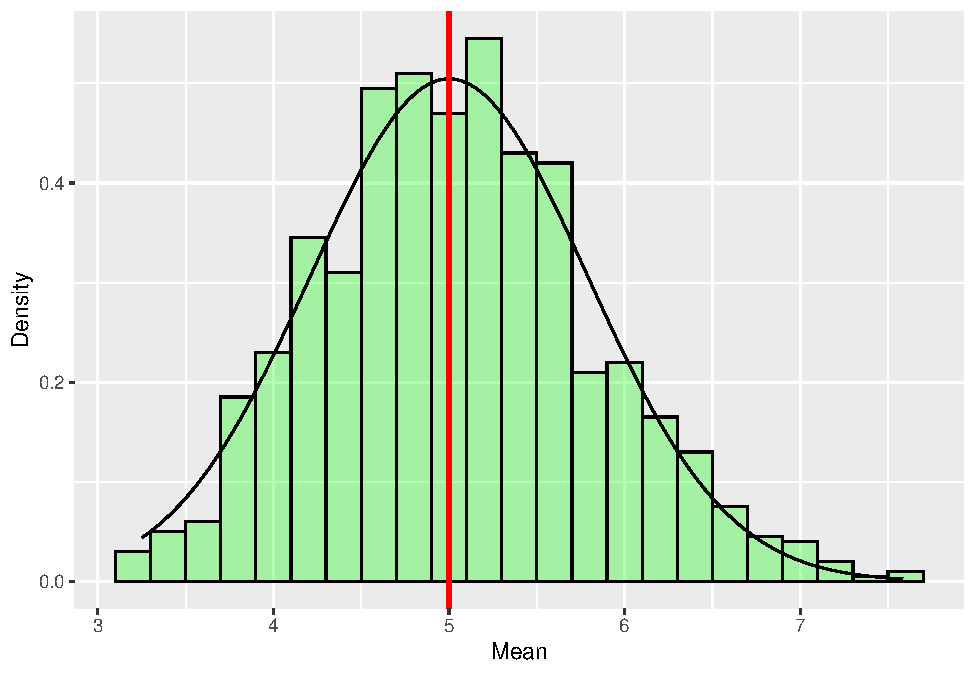
\includegraphics{StatsInf-Part1_files/figure-latex/unnamed-chunk-4-1.pdf}
In the figure above, we can see the CLT distribution from the green bars
and compare this distribution against the theoretical mean (vertical)
line. We can see that CLT is doing a pretty good job at estimating the
exponential distribution mean, given the sample set size and sample
count parameters.

Other observations from the figure is the tails of the distribution
curve appears non-continuous (gaps). In order for CLT to produce a more
``normal'' distribution, increasing the number of iterations can help
CLT avoid producing non-normal-looking distrubtions and avoiding gaps,
skew and kurtosis.


\end{document}
